\documentclass[tikz,border=1.35mm]{standalone}

\definecolor{fvmadaptedge}{HTML}{8A7E7E}

% Plain irregular six-sided face used as the general polygonal face example.
% Coordinates are in millimeters; y=-1mm keeps the SVG-style origin at top left.
\begin{document}
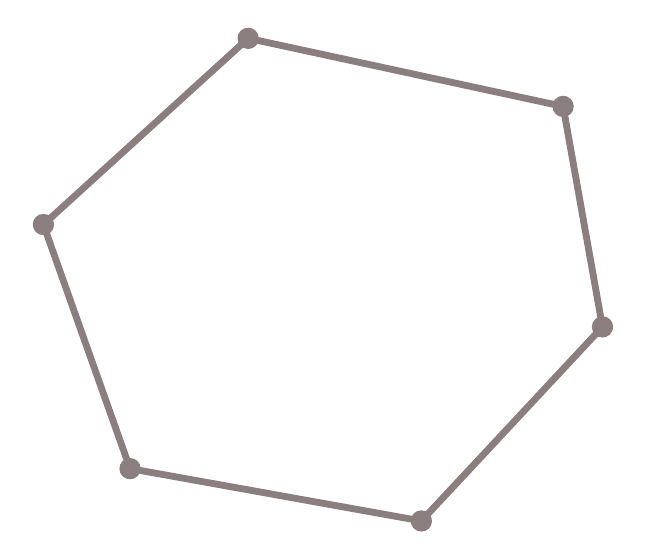
\begin{tikzpicture}[x=1mm,y=-1mm,line join=round]
  % Match the artwork frame before the standalone border is applied.
  \useasboundingbox (0,0) rectangle (76.000,64.000);

  % Irregular face vertices, ordered around the boundary.
  \coordinate (v0) at (28.000,1.353);
  \coordinate (v1) at (68.000,10.000);
  \coordinate (v2) at (73.000,38.000);
  \coordinate (v3) at (50.000,62.647);
  \coordinate (v4) at (13.000,56.000);
  \coordinate (v5) at (2.000,25.000);

  % Draw edges first so vertex markers sit cleanly on top.
  \draw[draw=fvmadaptedge,line width=0.865mm] (v0) -- (v1) -- (v2) -- (v3) -- (v4) -- (v5) -- cycle;

  % Original vertices are #8a7e7e.
  \foreach \p in {v0,v1,v2,v3,v4,v5} {
    \fill[fvmadaptedge] (\p) circle[radius=1.353mm];
  }
\end{tikzpicture}
\end{document}
